\documentclass[12pt,letterpaper]{article}
\usepackage{amsmath,amsthm,amsfonts,amssymb,amscd}
\usepackage{fullpage}
\usepackage{lastpage}
\usepackage{enumerate}
\usepackage{fancyhdr}
\usepackage{mathrsfs}
\usepackage{xcolor}
\usepackage{dsfont}
\usepackage{graphicx}
\usepackage[framed]{mcode}
\usepackage[margin=3cm]{geometry}
\setlength{\parindent}{0.0in}
\setlength{\parskip}{0.05in}

% Edit these as appropriate
\newcommand\course{CIS 581}
\newcommand\semester{Fall 2014}     % <-- current semester
\newcommand\yourname{Michael O'Meara, Mike Woods} % <-- your name
\newcommand\hwdate{Due: December 15, 2014}           % <-- HW due date

\newenvironment{answer}[1]{
  \subsubsection*{Our #1}
}


\pagestyle{fancyplain}
\headheight 25pt

\lhead{\\\course\ --- \semester}
\chead{\textbf{\Large Project Checkpoint \hwnum}}
\rhead{\hwdate}

\headsep 5pt

\begin{document}

\text{\yourname}

\begin{answer}{approach}

\begin{enumerate}

\item Our approach initially involved using the code published by Zhu and Ramanan based on a paper called "Face Detection, Pose Estimation and Landmark Localization in the Wild" to perform landmark detection on the input or reference faces. So far, one of most challenging sub-problems we've encountered has to do with obtaining a clear outline of the face, specifically the jawline. The code by Zhu and Ramanan performs this task fairly well in most test images we've tried.
 
\item Using the initial points, we then compute the convex hull of the faces in both images.  This allows us to calculate a polygonal mask of the reference image and an inverse mask of the target image.  We will later use both to extract the actual face from the input image and create a hole in the target image for adding the convex hull of the reference image. 

\item After trying many different approaches involving localized feature detection in order to match points with no real success, we finally found code published by Serge Belongie, Jitendra Malik and Jan Puzicha on matching point features using Shape Context.  Their code uses Hungarian Bipartite graph matching and gave us almost perfect point correspondence between the reference and target image as can be seen in our results on the next page.

%\item Additionally, we also construct a bounding box/region of interest based on the initial set of detected facial points which we use to perform localized feature detection, identifying the nose, eyes, and mouth. The location of the nose is also used to perform left eye/right eye disambiguation and remove false positives. 

%\item Our next task is to detect the best corners within the local feature bounding boxes (most likely on the eyes and mouth) of the source and target images in order to prune dissimilar correspondence points in both the target and source images. 

\item Now, our goal is to use those corresponding points from both images to do TPS morphing, repeating the previous steps until the points from both overlap to within some tolerance level.

\item Finally, we will use Laplacian blending to ensure a smooth transition from our face into the surrounding target image.

\end{enumerate}

\end{answer}


\begin{answer}{results}

\begin{figure}[!ht]
        \caption{Shape context point matching}
\center
%        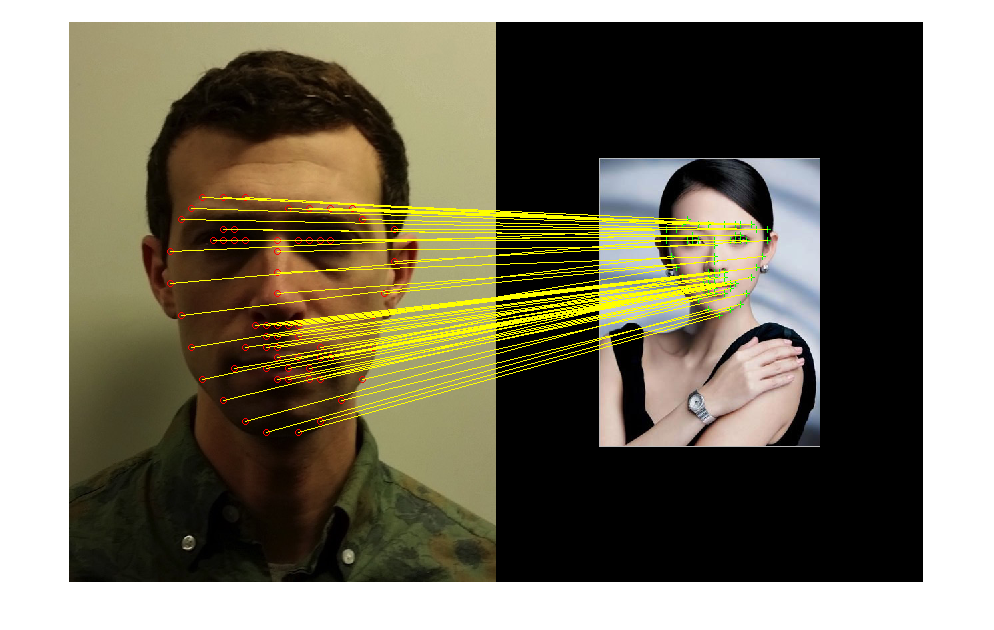
\includegraphics[scale=0.25]{match_1}
        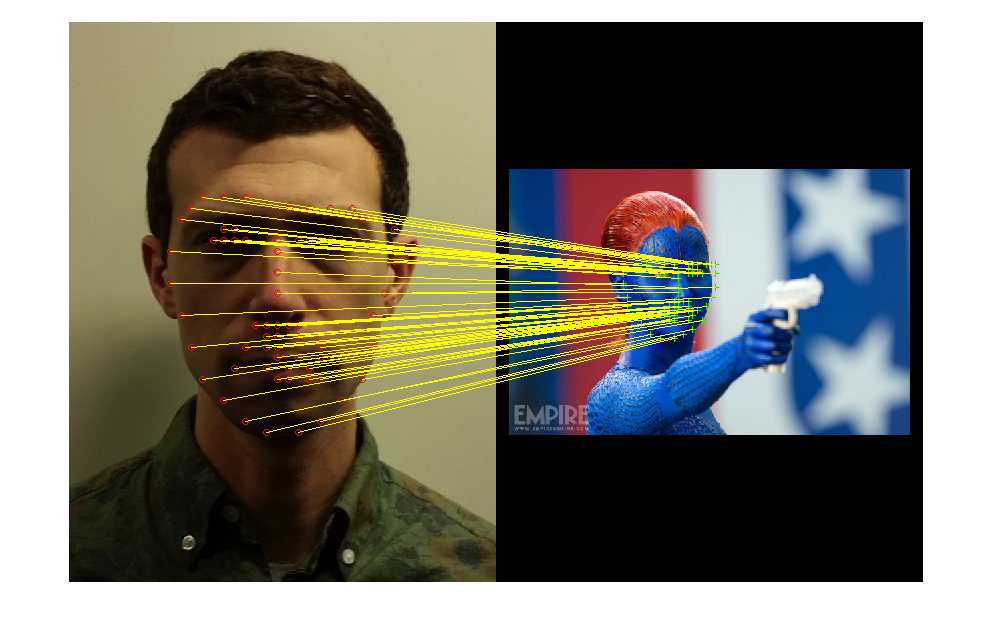
\includegraphics[scale=0.3]{match_2}
        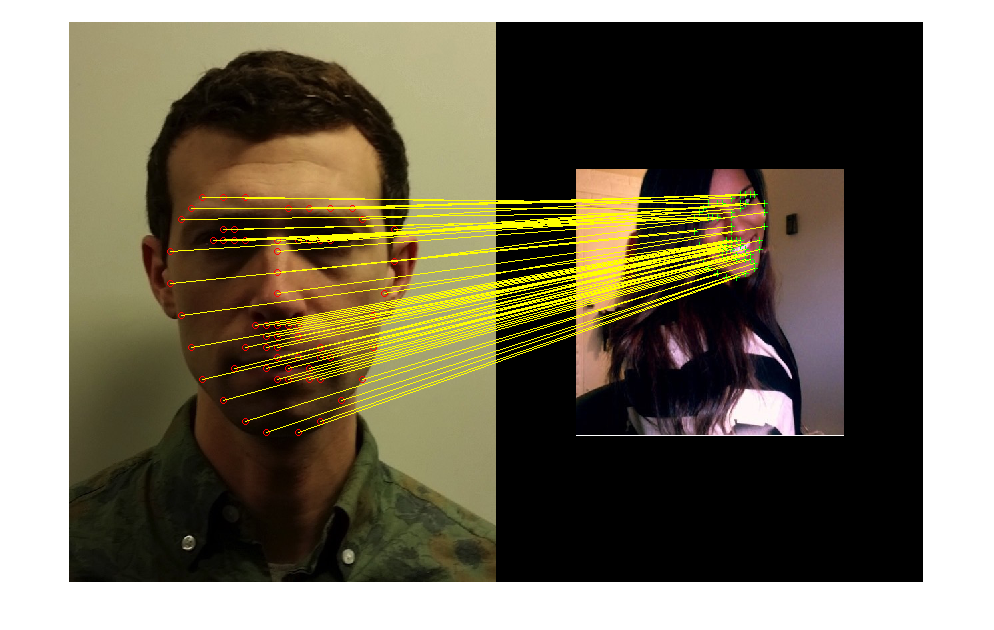
\includegraphics[scale=0.3]{match_3}
        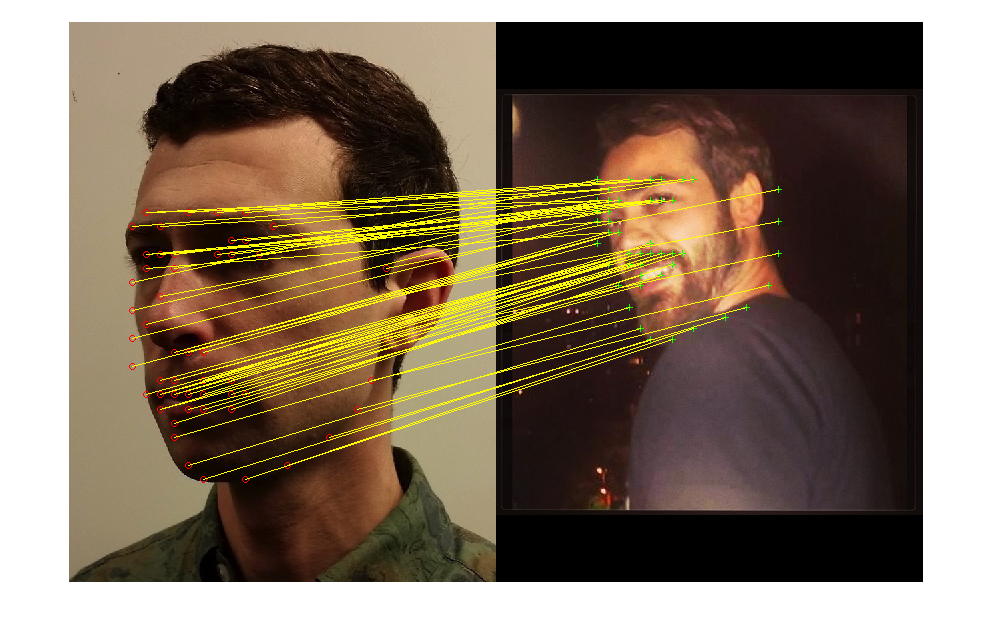
\includegraphics[scale=0.3]{match_4}
\end{figure}


\end{answer}


\end{document}


